\section{Single View Metrology (Height Estimation)}

\paragraph{Introduction} We consider an image of two people standing on the same ground plane (Figure \ref{fig:annotated_points}), annotated with:

\begin{itemize}
    \item Two pairs of parallel lines in the scene.
    \item Two points identifying a segment of known length, i.e. the reference height. 
    \item Two points identifying a segment of unknown length, i.e. the height to be estimated.
\end{itemize}

\begin{figure}
    \centering
    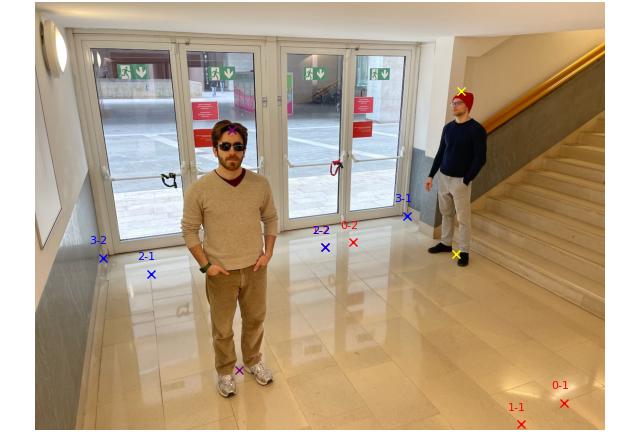
\includegraphics[width=0.5\linewidth]{img/annotated_points.png}
    \caption{In blue and red, the points identifying the two pairs of parallel lines. In yellow, the points representing the height to be estimated (Jack's). In purple, the the points representing the reference height (Dave's).}
    \label{fig:annotated_points}
\end{figure}

\paragraph{Notation} In this section, we use the following notation:

\begin{itemize}
    \item \textit{Person 1} (Dave): the person whose height is known and we use as reference.
    \item \textit{Person 2} (Jack): the person whose height is unknown and we want to estimate.
    \item $h_i$, $f_i$: the points identifying Person $i$'s height, for $i=1,2$.
    \item $p_{j,1}$, $p_{j,2}$: the points identifying the $j$-th parallel line annotated in the scene, for $j=1,2,3,4$.
\end{itemize}

\paragraph{Background} Our methodology heavily relies on a key property of projective geometry, which involves homogeneous coordinates and the cross product. Let $x,y,v,w \in\mathbb{P}^2$ be four points in the projective plane (our image) and let $\times$ denote the cross product in $\mathbb{R}^3$. Then the following holds:

\begin{itemize}
    \item $x \times y$ are the homogeneous coordinates in the dual projective plane of the line passing through $x$ and $y$. 
    \item $(x \times y) \times (v \times w)$ are the homogeneous coordinates in the projective plane of the intersection of the line passing through $x$ and $y$ with the line passing through $v$ and $w$.
\end{itemize}

\paragraph{Methodology} To estimate the height, we use the annotations to identify the pairs of parallel lines and their intersection points. We then compute the horizon as the line passing through these intersections. Then, we find the intersection of the line through the feet of the two people with the horizon. From this point, we draw a line to project the height of one person onto the other. Finally, we measure their ratio in the image reference system and use a proportion to retrieve the original height. More in details, we proceeded as follows.

\begin{enumerate}
    
    \item Extend the 2D coordinates of the points in the image reference system by setting the third coordinate to $1$ to get the homogeneous coordinates and identify the parallel lines (Figure \ref{fig:retrieved_lines}):
    \begin{align*}
        l_{parallel_j} &= p_{j,1} \times p_{j,2} \quad \text{with }j=1,2,3,4\\
    \end{align*}

\begin{figure}
    \centering
    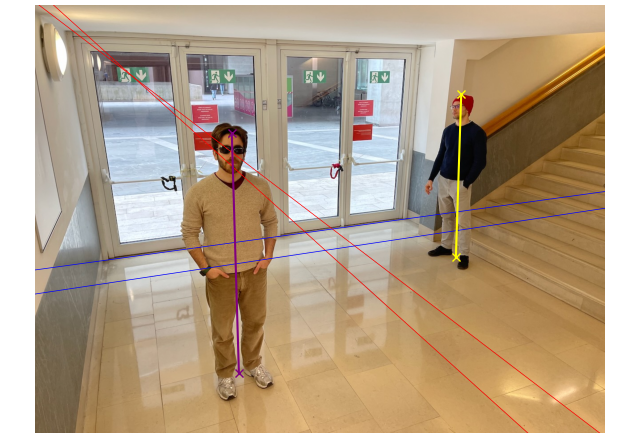
\includegraphics[width=0.5\linewidth]{img/retrieved_lines.png}
    \caption{In blue and red, the lines retrieved using the annotated points and the cross-product property. In yellow and purple, the segment representing the height of the person. The purple segment is true length is known, the yellow is the one we estimated.}
    \label{fig:retrieved_lines}
\end{figure}
    
    \item Identify the vanishing points and the horizon (Figure \ref{fig:wide}):
    \begin{align*}
        v_{left} &= l_{parallel_1} \times l_{parallel_2}\\
        v_{right} &= l_{parallel_3} \times l_{parallel_4}\\
        l_{\infty} &= l_{parallel_1} \times l_{parallel_2}\\
    \end{align*}

\begin{figure}
    \centering
    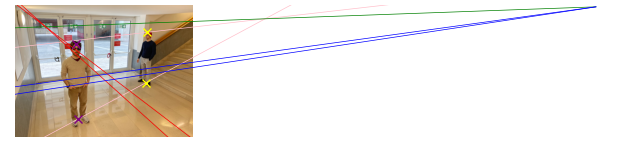
\includegraphics[width=0.6\linewidth]{img/wide.png}
    \caption{In green, the retrieved horizon. The left and right vanishing points are represented by the intersection of the horizon with the red lines and blue lines respectively.}
    \label{fig:wide}
\end{figure}

    \item Identify the line passing through the feet $f_1$ and $f_2$ of the two people (Figure \ref{fig:final}:):
    \begin{align*}
        l_{feet} = f_{1} \times f_{2}
    \end{align*}
    
    \item Find the point at infinity by intersecting $l_{feet}$ with the horizon (Figure \ref{fig:final}:):
    \begin{align*}
        p_{\infty} = l_{feet} \times l_{\infty}
    \end{align*}

    \item Project the second person's height onto the line $l_1$ where the reference person's height segment lies (Figure \ref{fig:final}):
    \begin{align*}
        l_{1} &= t_1 \times f_1 \\
        l_{heads} &= p_{\infty} \times t_2 \\
        t_2^{\prime} &= l_{heads} \times l_{1}
    \end{align*}

    \item Normalize the projected point to get the coordinates in the image reference system:
    \begin{align*}
        t_2^{\prime} = \frac{t_2^{\prime}}{(t_2^{\prime})_3}
    \end{align*}

    \item Calculate the height ratio and estimate the true height $\hat{h}^*_2$ using the annotated height $h^*_1$ (Figure \ref{fig:final}:):
    \begin{align*}
        h_1 &= \|t_1 - f_1\| \\
        h_2^{\prime} &= \|t_2^{\prime} - f_1\| \\
        \hat{h}^*_2 &= \frac{t_2^{\prime} \cdot h^*_1}{t_1}
    \end{align*}
    
\end{enumerate}

\paragraph{Implementation} The algorithm was implemented in Python using NumPy for matrix operations and PIL for image handling. We produced reference points in the image manually with our own-developed file \textit{annotator.py} – which is included in the source code and fully reproduceable – and stored their pixel coordinates in a text file.

\paragraph{Results} We tested our approach on an image where the actual height of the second person was known to be 184 cm. Using a reference person with a height of 175 cm, our algorithm estimated the second person's height to be 184.10 cm.

\paragraph{Discussion} On this particular image, the final result was extremely precise. However, we noticed that it is very sensitive to small shifts in the annotations, and on different test images it performed slightly worse. For example, we considered an image where the left vanishing point was extremely close to one person's reference points, which greatly magnified annotation errors and resulted in suboptimal results. Additionally, we noticed that using two pairs of parallel lines as references in the scene such that two non-parallel lines intersect at an annotated point (point $2,2$ in Figure $1$) significantly improved the estimation accuracy.  

\begin{figure}
    \centering
    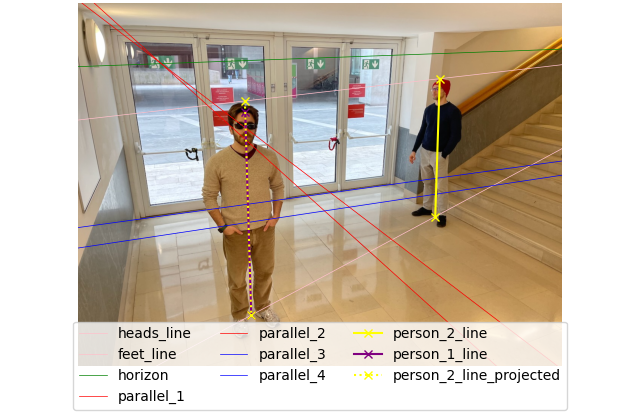
\includegraphics[width=0.5\linewidth]{img/final.png}
    \caption{The final result. The purple line (Person 1's height) is known to be 175 cm in reality. The yellow line (Person 2's height) is estimated to be 184.10 cm in reality (true is 184 cm). The dashed yellow line represents the projection of the yellow line onto the purple line.}
    \label{fig:final}
\end{figure}